% Changing book to article will make the footers match on each page,
% rather than alternate every other.
%
% Note that the article class does not have chapters.
\documentclass[letterpaper,10pt,twoside,twocolumn,openany]{book}

% Use babel or polyglossia to automatically redefine macros for terms
% Armor Class, Level, etc...
% Default output is in English; captions are located in lib/dndstring-captions.sty.
% If no captions exist for a language, English will be used.
%1. To load a language with babel:
%	\usepackage[<lang>]{babel}
%2. To load a language with polyglossia:
%	\usepackage{polyglossia}
%	\setdefaultlanguage{<lang>}
\usepackage[english]{babel}
%usepackage[italian]{babel}
% For further options (multilanguage documents, hypenations, language environments...)
% please refer to babel/polyglossia's documentation.

\usepackage[utf8]{inputenc}
\usepackage{hang}
\usepackage{lipsum}
\usepackage{listings}
\usepackage{graphicx}

\usepackage{dnd}

\lstset{%
  basicstyle=\ttfamily,
  language=[LaTeX]{TeX},
}

% Start document
\begin{document}


	\chapter{Agdha Zacharias}
	
	
	\begin{figure}
		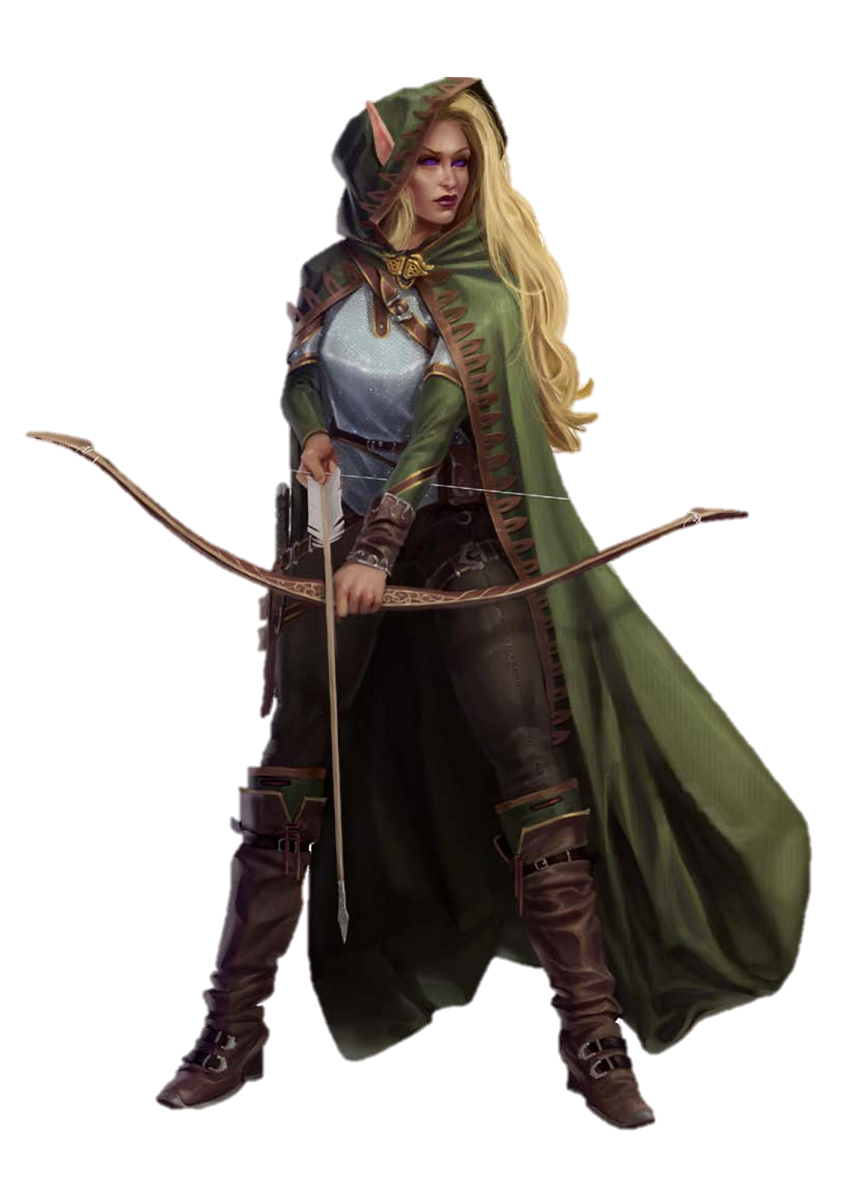
\includegraphics[width=\linewidth]{../elfranger3.png}
		\label{fig:az}
	\end{figure}


	\begin{quotebox}
		Nobody can teach you better than nature, it has been doing so for years.
	\end{quotebox}
	
	
	
	\header{General Information}
	\begin{dndtable}
	
		Race  & Half-Elf \\
		Class  & Ranger \\
		Background  & Outlander \\
		Alignment & Chaotic Neutral \\
		Age & 34 \\
		Origin & Forester \\
		Conclave & Beast Conclave
	\end{dndtable}
	
	\vfill\null

	\section{Background}
		\subsection{Traits}
		Nature raised me, and I have still so much to learn. I want the others to learn the ways of nature as well as they are my friends. I will never pass a chance to teach a lesson about nature. 
		\subsection{Ideal}
		People come and go, their structures as well. They are unimportant in the timeline of the world. What must be protected is the fields and trees, bushes and lakes, rivers and mountains that nature provides. 
		\subsection{Bond}
		One of the few ways to make me an enemy is, … well either kill my whole hometown which has been done before or injure what hurts me most – nature. 
		\subsection{Flaw}
		If you don’t know how to survive out there, no worries I’ll help you. But if you are useless out there you better just stay where you are because bears like a nice snack from time to time. 

	\pagebreak
	
	\section{Story}
	\subsubsection{Early Years}
	The town I was born in was idyllic and quiet. One of the few places in this world where it didn’t matter what race you are and where you come from as long as you were nice to everyone else. My father was an elf, my mother human. I don’t know how the two found each other but I know that my father was thrown out of his clan when they found out. My mother was already pregnant and out of sheer luck they found this little town to live in. My first years were great. My father and I often went on camping trips in the nearby forest. He teached my how to use the longbow and which plants were edible or not. I had a blast back then. Young and naïve I was, I didn’t even know that there’s a war going on on the other side of the forest and that people like me are not welcome in this world. “The empire”, my father used to say, “do not like young half elves like you but don’t worry.”. 
	
	But our idyllic way of living was not for long. One day the soldiers of the empire marched into our city. My father sent me away and after some protesting I gathered my stuff and ran off into the woods, alone. After a week I returned to our town which was now a place of ash and burned corpses. The empire destroyed everything I had. 
	
	\subsubsection{The Woods}
	I started to live in the woods. I was young and even though I went camping a lot I wasn’t prepared. There are beasts in the forest I do not dare speak of. Nature seemed to work against me no matter what I did. I frequently went on for several days without finding any food. Everything changed one day. There were three goblins near my camp. I overheard them say that the ground they stood on was perfect for their clan to reside. They started by making a campfire, which was fine, but soon ignited some torches and buring down foilage, trees and bushes around them. They were about to destroy the forrest for their own means! I quickly grabbed my longbow and climbed on a tree. I shot them down with three arrows. I’ve never been angrier at that point and never been this precise. I put out the already buring fire with my bare hands and stayed there to make sure that there are no other goblins approaching.
	
	After this incident the way nature treated me changed. It seemed like nature was starting to respect me after I had saved it from burning down. Even the animals were nicer towards me. I got along well with the smaller ones and they would alert me if there was a predator on the way. I protected the forest and the forest protected me. 
	
	\subsubsection{Mentor}
	The first lession nature teached me was just a couple of days after the goblin incident. It was night and a little bug crawled on my face. I woke up. This was the first time I felt unwell in the woods. Something wasn’t quite right. I snuck out of my campsite and wandered around as quietly as I could. But my feet seemed to be louder than usual on the forest floor. I heard each leaf I stood on. Soon I realized what was wrong. The forest was dead silent. Not a single bug or bird was to be heard. I stood still in my tracks and started to listen more carefully, after I managed to ignore my own breath I heard an eerie sound. Like someone mimics wind with their own mouth far in the distance. I jumped behind the closest tree and sat down. Trying to be as silent as possible. I observed some moonflowers, which bloom at night, close their leaves and face downward. This was highly unusual. After a few more minutes I saw what they were turning against from. A dark creature, much like a shadow, was passing through the woods. About 500ft away from me. I held my breath trying to make no sound at all. When the flowers were not facing the creature, why should I? The shadow creature went further away. The weird thing was, it passed through the trees as if they weren’t there. I sat by that tree until the morning sun arrived and the flowers around me started blooming again. That was the night I learned that nature knows so much more than we do. 
	
	\subsubsection{Animals}
	The woods were very lonely at times. I sometimes feared that I'll soon forget how to speak. That's probably why I bond with animals so much. The smaller ones often slept near me and played with me during my younger years. If one was hurt they'd lead me to it and I'd try my best to get it back on track. Sometimes I feel I could speak with them, read their minds. I mostly know exactly what these creatures want. I adapted to them. But most animals in the woods have a short life span and it broke my heart everytime I lost a little friend. 
	
	\subsubsection{Challenges}
	After about 15 years in the woods I decided it was time to go out and meet some other beings than animals. I've seen many towns near the edge of the forest and went to the one that I had deemed most safe. It felt really weird being around people but my fear that I forgot how to speak soon proved itself wrong. I got along with the people there. Problem was that I had no money and couldn't just sit with them and have a drink. Some human must have realized this and offered me a little "challenge" as he called it. He bet me that I could not shoot a specific apple off the nearest tree. I took that challenge and asked him which apple he wants. As he was pointing to it I quckly drew my longbow and shot away. The apple fell on the ground - in it my arrow. I got to keep the apple and he gave me some metallic coins. He told me that would be enough to have a drink at the bar with him. He introduced himself as Arno.  
	
	In the bar we talked about our past lives. The human had a rather boring life but I learned that he was quite rich. I didn't really care for human wealth but after a while of pretending to, he offered me a job at his mansion. He has pissed someone off and wanted me to protect the house while he sleeps until the danger is over.
	 
	I took the job. He offered me a guest room to sleep in during the days but it was really uncomfortable and I felt trapped in that little room. After that I slept outside. 
	
	Arno told me more about this other guy. Apperiantely it was a goblin that was living in a cave Arno owns. Arno tried to throw the guy out so he could use the cave as secure storage but the goblin, which goes by the name Blacks, would not move. So Arono flooded the cave out of despair. Blacks got out but screamed murder. Arno later learned that Blacks was a hitman and was now after him. 
	Many nights went by without something happening. But one night Blacks finally showed up. He must have learned my walking patterns and got to the mansion unnoticed. I only realized he's there because he had to break the door and I happend to heard that. I chased him into the mansion and we fought. It was a hard fight but in the end I was able to stab Blacks in the heart with my shortsword. 
	
	Arno payed me a lot of coins and I went on, switching between living in the woods and doing small jobs for strangers. 
	
	\subsubsection{Striking back}
	One day while making my rounds in the woods a little squirrel approached me. It was furios, would climb up and down my cape and I felt it wanted me to follow it and so I did. The squirrel ran through the forest, then through fields and through rivers. It was hard to keep up, but I felt it was important. Soon I saw black smoke rising from a little town in the distance. I saw soldiers much like the ones that invaded my little hometown. Suddenly I was even more furious than the squirrel and overtook it. In the city, which I later got to know as “Goldfield” was a huge fight going on. Empire against the common people. It wasn’t hard to decide which site to root for. I shot some arrows from the distance, it may hit one or two soldiers, but they were stronger than the goblins back then. In the middle of the city there was a group of people from different races together fighting. I really liked the view of them uniting against the greater force and joined them in the fight. There was a gnome, another half-elf and even a tiefling. 
	
	After a lot of fighting and many causalities on our side, victory was ours. The last soldiers of the empire were either dead or fleeing the city. The other adventurers were as happy as I was. Later, in the middle of celebration, I noticed the little squirrel on the gnome’s shoulders. 
	
	




		
		
		

	
% End document
\end{document}
